\chapter{Background}

% Introduce what is planning under uncertainty
Planning and reasoning under uncertainty is central to robotic and artificial intelligence research and has 
been an active area of research for decades. It is an umbrella term which touches a
wide spectrum of fields: \textit{economics}, \textit{psychology}, \textit{cognitive science}, \textit{neuroscience},
\textit{robotics} and \textit{artificial intelligence}. The work in this thesis relies on results  and assumptions 
made in cognitive and neuroscience with respect to our beliefs and how we act given them. We complement 
these results by introducing them in a new light to the field of robotics and demonstrate how the human reasoning and belief system 
can be used in situations where the state space is partially observable. The second main theme our work builds on is 
state space estimation. The third component acting given uncertainty in robotics. We make use of results from all 
three fields. We provide a background overview of acting under uncertainty and situate our work within the state of the 
art.

This chapter unfolds as follows: 



\section{Decisions under Uncertainty}
% What is the the reasoning under uncertainty planning problem
% What are all the assumptions which can be made regading the belief

In this section we introduce and frame the problem we seek to solve in generic 
terms. We are concerned with finding a sequence of actions which will lead to the successful 
outcome of a problem being considered; this is the most generic definition. 

There are two key attributes which can make this problem difficult: stochastic actions and latent states. Stochastic 
actions, when applied in the same state will not always result int the same outcome. This type of uncertainty 
can arise from many sources; the outcome of chaotic actions are impossible to predict with certainty, 
think of throwing a die or flipping a coin; In outdoor robotics the terrain might lead to slippage, causing 
the robot to skid or underwater currents might drastically offset the position of an UAV; In articulated 
robots the friction between joints can accumulate to a large error in the end-effector position (especially true 
for cable driven robots). 
The second source of uncertainty is when the underlying state is partially known, in the sense that we do not 
have all the necessary information to reliably determine the state beyond reasonable doubt. In robotics this 
uncertainty can arise from inadequate or noisy sensors. If the environmental conditions in which the robot 
is located is humid, misty or dark. It can make it difficult for the robot to ascertain its position and 
to plan how to achieve a given objective.

The uncertainty of the state and actions have to be quantified. The predominant approach 
is to  represent them by probabilities. For instance the application of a forward action (for a wheeled robot) 
will result in a new position further ahead and a position to the right (due to slippage) with some probability.
An observation through the robots sensors will result in probability distribution over the robots probable location.
Given this quantification of action and observation uncertainty in terms of a probability distribution over the state, 
the agent must now take actions towards accomplishing its goal. To take a decision the agent must assign a utility 
to the outcome of his actions. The utility is to indicate a preference over the outcomes and when combined with 
probabilities leads to decision theory. 

\subsection{Decision theory}

The central question of decision theory is; \textit{how do we take decisions when faced with uncertain outcomes ?} To answer
such a question we need to ground the attributes which are involved when we take a decision, namely our \textbf{beliefs} and 
\textbf{desires}. Beliefs reflect a degree of knowledge we have about the world in which the degree is ascertained by 
the amount of evidence we have in support of our beliefs. Epistemology studies in great detail the relationship between 
truth, beliefs and knowledge. We will not go into a philosophical discussion of their interplay, but make use of the following; 
if we have sufficient evidence in support of our beliefs and they represent the truth then we consider them to 
be a \textbf{rational belief}. As for desires they are linked to our disposition to take action to achieve them; for 
example if I want to switch of my alarm clock I have to look for it in the last area I believed it to be. 
These two attributes, beliefs and desires, are used to frame a decision problem. Early work in decision theory assumed 
that the problem was well grounded and focused on finding what are the \textbf{rational choices} to take given our beliefs 
to achieve our desires. 

\begin{figure}
 \centering
 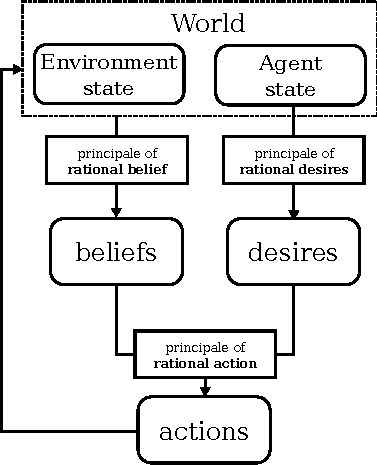
\includegraphics[width=0.5\textwidth]{/home/guillaume/Documents/Thesis/ch2-Background/Figures/cognitive_loop.pdf}
  \caption{ad}
\end{figure}

Early interest in such questions were typically centred around economics such as deciding what should be an appropriate 
investment or wager for a particular gamble. It was noted that the expected monitory outcome of a gamble as a mean of basing a 
decision, would often lead to a course of action which contradicts common sense; a famous example is the St. Petersburg paradox.
In this paradox a bookmaker proposes you the following gamble. An initial pot starts with a content of 2\pounds, the bookmaker proceeds 
to flip a fair coin until the first appearance of a tails which ends the game. Until the occurrence of the first tails 
the money in the pot doubles after every toss. Once the game ends you leave with the content of the pot. As an avid gambler 
and expected value maximiser how much would you be willing to pay to enter this gamble ? A value maximiser would computed 
the expected monetary outcome. The amount of money increases by $2^{n}\pounds$, where $n$ is the number of non-final tosses and 
and the probability of reaching $n$ is $1/2^{n}$. In this case the expected monitory outcome is an infinite number,

\begin{equation*}
\displaystyle \mathop{\mathbb{E}}_{p(n)}\{\pounds\} = \underbrace{\frac{1}{2} 2 \pounds}_{\textrm{first toss}} + \frac{1}{4} 4 \pounds + \dots = \sum\limits_{n=1}^{\infty} 
\frac{2^{n}}{2^{n}}\pounds = \infty \pounds 
\end{equation*}

So your expected gain or return for paying to enter such game is an infinite amount of money, so in principal if you were
seeking to maximise your expected return value you would be willing to pay an amount close to infinity. This does not 
seem a good decision rule; no person in the world would be willing to pay more than $1\pounds$ to enter such game.

Nicola Bernoulli proposed a solution to the problem (later published by his brother Daniel  (\cite{Bernoulli1954})) by introducing the notion 
of a \textbf{utility function}, and he claimed that people should base their decision on the expected utility instead 
of solely the monetary outcomes of a gamble.

\begin{quote}
  \onehalfspacing% <--- Local line spacing
  ``...the value of an item must not be based on its price, but rather on the utility it yields."\par\raggedleft--- \textup{Daniel Bernoulli}
\end{quote}

The introduction of a utility function takes into account that the net worth of a person will influence their decision since 
different people (in terms of their monetary worth) will weigh the gain differently. The utility function introduced by Bernoulli 
was the logarithm of the monetary outcome $x \in X$ weighted by their probability $p(x)$ which results in an expected utility, 

\begin{equation*}\label{eq:exp_utility}
  U(x) = \displaystyle \mathop{\mathbb{E}}_{p(x)} \{ u(x) \} = \sum_{x\in X} p(x) \underbrace{\log(x)}_{u(x)}
\end{equation*}

Different utility functions characterise different levels of risk. When the it is concave as it for Bernoulli's utility function
the person will be \textbf{risk-averse}, when linear \textbf{risk-neural} and convex \textbf{risk-seeking}. 
This was the first introduction of a utility function.

It is later in 1944 that von Neumann and Morgenstern (\cite{VonNeumann1944}) axiomised Bernoulli's utility function 
and proved that if a decision maker has a preference over a set of lotteries\footnote{the term lottery refers 
to a probability distribution in the original text.} which satisfy four axioms
(completeness, transitivity, continuity, independence) then there exists a utility function who's expectation 
preserves this preference. An agent whose decisions can be shown to maximise the vNM expected utility are said 
to be \textbf{rational} and otherwise \textbf{irrational}.  This is the theoretical basis of most economic theory,
it is a \textbf{normative} model of how people should behave given uncertainty. It is also the basis of most 
if not all decision making, cogitative architectures and control policies in AI and robotics 
(to the best of the authors knowledge).

An aspect to keep in mind regarding the vNM model is that it is normative; it states what should be a rational decision 
or behaviour. As a result it is not always consistent with human behaviour. There is great debate regarding 
the predictions made by vNM models with respect to ours. There have been many studies both demonstrating divergence 
between the models predictions and our observed behaviour but also supporting evidence that it does reflect 
the output of our decision making process. Reasons for divergence have been attributed to the way we 
weigh probabilities and how the decision problem is framed. But probably the most important aspect is that 
in most decisions we are faced with the quantification and rationality of our beliefs might not be adequate
and limitations of our working memory will come into play in the final decision.

Nevertheless vNM agents are predominantly used in AI and robotics as a means of implementing 
a decision making process or a control policy. In psychology and cogitative science vNM agents
are a used for comparing human behaviour against an optimal strategy (by optimal we mean it is rational in 
the vNM sense). 

%(see prescriptive models(\cite{Kahneman79prospecttheory}). 

% vNM is concerned with a one shot only decision, but what if we have to take a sequence of decisions ? What 
% happens then ?

%How is the uncertainty quantified ? Answer: probability theory
%How does the agent make a decision ? He must assigned a preference to the outcome of various actions
%Utility theory and combined with probability lead to decision theory.

% Speak about the historical context of plannig un
% Uncertainty and rational actions


% vNM theorem is limited to evaluation options that come with an 
% objective probability distribution over outcomes.
% a situation decision theoriests and economists often describe 
% as ''choice under risk``

% The utility function represents the agents desires.
% so the probability function represents her beliefs.
% The theories are referred to collectively as subjective expected utility (SEU).

% How is decision theory used in robotics ?


\subsection{Beliefs \& desires}

% POMDPs provide a rich framework for sequential decision-making under uncertainty in stochastic domains.
% Solving a POMDP is often intractable.

%\begin{enumerate}
% \item Decision theory
% \item Markov Decision Process
% \item Partially Observable Markov Decision Process
%\end{enumerate}

\begin{table}
\begin{center}
\renewcommand{\arraystretch}{1.5}
\begin{tabular}{|l|p{9cm}|} 
\hline
    \textbf{Notation} 			 	& \textbf{Definitions} \\ \hline\hline
    $x_t \in \mathbb{R}^3$ 		 	& Cartesian state space position of the agent.\\
    $y_t \in \mathbb{R}^{M}$		 	& Observation/measurement from the agents sensors.\\
    $a_t \in \mathbb{R}^3$		 	& Action, usually the Cartesian velocity of the end-effector of the agent.\\
    $X,Y,A$				 	& State, observation and action random variables where $x$, $y$ and $a$ are realisation.\\
    $p(x_t)$ 					& Short hand notation for a probability density function, $p_{X}(x_t)$.\\
    $x_{0:t}$					& $\{x_0,x_1,\cdots,x_{t-1},x_t\}$, history up to time $t$.\\
    $p(x_t|y_{0:t},a_{0:t})$	 		& Filtered probability distribution over the state space given the action and observation history.\\
    $b_t \in \mathbb{R}^{L}$			& Belief state, a function of the filtered distribution 
						 $b(p(x_t|y_{0:t},a_{0:t}))$ which will be written as $b_t$ for simplicity.\\
    $\policy(a_t|\cdot)$ 				& Probabilistic policy, $a_t \sim \pi_{\boldsymbol{\theta}}(a_t|\cdot)$ \\
    $r(x) \in \mathbb{R}$			& Reward function, returns the utility of being in state $x$. It can also be dependent on the action, $r(x,a)$.\\
    $\gamma \in [0,1)$				& Discount factor, the closer to one the more later utilities/rewards are considered. When set to zero, only immediate rewards are 
						  considered which would result in a myopic greedy agent.\\
    $p(x_{t+1}|x_t,a_t)$			& State transition function, returns the likelihood/probability of reaching state $x_{t+1}$ given that action $a_t$ is applied in state $x_t$.\\	
    $p(y_t|x_t)$				& Observation/measurement model, returns the likelihood/probability of observing $y_t$ given that the agent is in state $x_t$.\\
    $\tau(b_{t-1}(x),u_{t-1},y_t)$		& Updates a belief given a motion and observation, it makes use of both the motion and observation functions. The state space estimation function, $\tau$, can be any kind of state space filter such as an Extended Kalman Filter (EKF) or a Particle Filter (PF).
    \\ \hline
\end{tabular}
\end{center}
\caption{Definition of common variables used.}
\label{tab:notation}
\end{table}


\section{Sequential decision process}

When referring outright to decision theory with no extensions, we usually are talking about a one-shot
non-temporal decision. However many interesting decision problems are sequential.
In such a situation we must consider the effect current decisions will have on future decisions. Expected utility 
theory (part of decision theory) is extendible to a temporal decision problem. There are however a two subtle but important 
differences between the temporal and non-temporal decision problems. The first is the utility, in the one time step problem 
an outcome has one utility assigned to it, $u(x)$. Now a utility has to be assigned to a sequence of outcomes, $u(x_{0:T})$, 
where $T$ is the number of sequential decisions taken. The utility of a sequence is the sum of the individual outcomes 
themselves. However if the decision problem is non terminating this will lead to an unbounded utility. To bound the utility a 
discount factor $\gamma \in [0,1)$ is introduced and the new utility function becomes:

\begin{equation}
    u(x_{0:T}) 	   = \sum\limits_{t=0}^{T} \gamma^{t} u(x_t) \label{eq:joint_state_actions_util}
\end{equation}

The discount factor allows to control the importance later utilities have on the final utility. If the discount factor is set to
zero we recover the original one-shot utility function and if we were to take actions which maximised the expected utility 
we would not be considering at all the effect later decisions have on our overall utility. An agent reasoning in such a way is 
called myopic.
The second is the way in which probabilities are assigned to outcomes, this was $p(x)$ in the decision theory utility function formulation.
Now because of the sequential nature of the problem we consider a conditional state transfer probability distribution $p(x_{t+1}|x_t,a_t)$
which models the probability of going from state $x_t$ to $x_{t+1}$ given that action $a_t$ is taken. This particular representation of a
sequential decision problem is called a \textbf{Markov Decision Process (MDP)} and to be more exact a first order MDP.
The necessary models are the state transition and utility functions. The assumption of such a model is that all necessary information to 
take a decision is encoded in the current state and there is no need to consider the history of state transitions when taking a current decision.
In Figure \ref{fig:mdp} we illustrate two graphical representations of a MDP, which are known as \textbf{Dynamic Bayesian Networks (DBN)}.
A DBN represents the the temporal relationship and conditional dependence between random variables, decisions and utilities, which are 
represented by circles, squares and diamonds. For the MDP to the left the actions are not stochastic, whilst for the MDP on the right 
the actions taken are governed by a stochastic \textbf{policy}, $\policy(a_t|x_t)$. A policy represents the decision process of an agent,
given a state it will output an action. A stochastic policy means that given the same input they will produce
different outputs. A policy is considered optimal when it maximises the expected utility function, it is optimal in the vNM sense.

\begin{figure}[h]
  \centering
  \subfigure[off-policy]{\label{fig:mdp_off}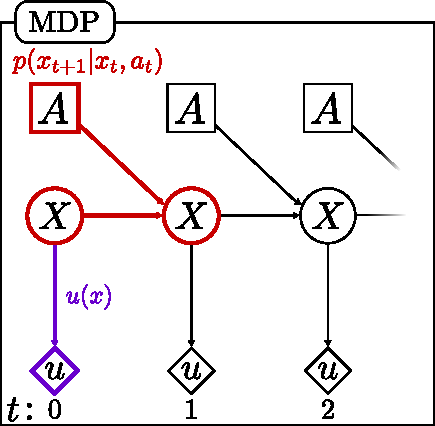
\includegraphics[width=0.45\textwidth]{/home/guillaume/Documents/Thesis/ch2-Background/Figures/mdp3.pdf}}
  \subfigure[on-policy]{\label{fig:mdp_on}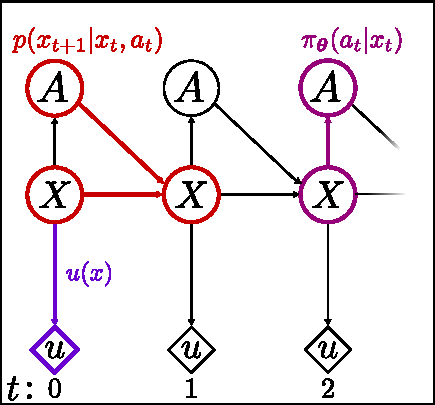
\includegraphics[width=0.45\textwidth]{/home/guillaume/Documents/Thesis/ch2-Background/Figures/mdp2.pdf}} 
  \caption{Dynamical Bayesian Network of a Markov Decision Process; it encodes the temporal relation between the random variables (circles),
  utilities (diamond) and decisions (squares). The arrows specify conditional distributions. In \textbf{(a)} the decision nodes are not considered 
  random variables whilst in \textbf{(b)} they are. From these two DBN  we can read off two conditional distributions, the state transition distribution (in red) and the action distribution (in purple). }
    \label{fig:mdp}
\end{figure}

Solving a MDP means finding a policy whose actions in any given state will always maximise the expected utility. Such 
a policy is usually denoted as $\pi^*$, the optimal policy. As in decision theory, the expected utility is the utility 
of  a sequence of states $u(x_{0:T})$ weighted by its probability . The graphical representation allows to read off directly the probability 
of a sequence of state transitions and actions $(x_{0:T},a_{0:T-1})$, Equation \ref{eq:joint_state_actions}.
\begin{align}\label{eq:joint_state_actions}
  p(x_{0:T},a_{0:T-1}) &= p(x_{0}) \prod_{t=0}^{T-1} p(x_{t+1}|x_t,a_t) \\
  u(x_{0:T}) 	       &= r(x_0) + \gamma r(x_1) + \dots + \gamma^{T-1} r(x_{T-1})  + \gamma^T r(x_T)
\end{align}
We are interested in finding the sequence of action, $a_{0:T}$, which will maximise the expected utility function:
\begin{equation}\label{eq:temporal_expected_utility}
 \argmax_{a_{0:T-1}} U(x_{0:T},a_{0:T-1}) = \max_{a_0} \sum\limits_{x_1}   \cdots  \max_{a_{T-1}} \sum\limits_{x_T} \Bigg( p(x_{0:T},a_{0:T-1}) u(x_{0:T}) \Bigg)
\end{equation}
Solving the above directly in its current form would have an exponential complexity. By making use of the first order 
markov assumption and that current rewards do not dependent future rewards, the sums in Equation \label{eq:max_util} can be re-arranged and 
and recursive patter will emerge which we can take advantage off. Lets start from the last time step and move out of the sum all elements 
which do not depend on $T$ and $T-1$, which results in Equation \ref{eq:expansion}
\begin{align}\label{eq:expansion}
 &\argmax_{a_{0:T-1}} U(x_{0:T},a_{0:T-1}) =\max_{a_0} \sum\limits_{x_1}   \cdots  \max_{a_{T-2}} \sum\limits_{x_{T-1}} p(x_{0:T-1},a_{0:T-2})  \nonumber\\
 &\left( u(x_{0:T-2}) + \gamma^{T-1} \left( r(x_{T-1}) +  \gamma \max_{a_{T-1}} \sum\limits_{x_{T}} p(x_{T}|x_{T-1},a_{T-1}) r(x_{T}) \right) \right)
\end{align}
From the rearrangement we notice that Equation \ref{eq:expansion} has the same functional form as Equation \ref{eq:temporal_expected_utility}, 
except that the recursive component can be summarised by Equation \ref{eq:bellman}, which is known as 
the \textbf{Bellman} optimal equation.
\begin{equation}\label{eq:bellman}
 V^*(x_t) := r(x_t) + \gamma \max_{a_t} \sum\limits_{x_{t+1}} p(x_{t+1}|x_t,a_t) V(x_{t+1})
\end{equation}
For the terminal state $V_T(x_T) = r(x_T)$. The bellman equation is a means of solving a sequential decision problem 
through use of dynamic programming. It says the the utility of the current state is based on the immediate reward and 
the discounted maximum utility of the next state. Making use of this recursion reduced the computation complexity is 
quadratic in the number of states, $\BigO(T\, |A|\, |X|^2)$. To find the optimal value and subsequent policy an approach 
would be to repeatedly apply the bellman equation to each state until the value function converges. What makes the problem 
hard to solve is maximisation over the actions. This induces two problems, the first is that the optimisation is nonlinear 
and the second is that if the action space is continuous the maximisation will be expensive to compute.
This brings use to the two main approaches to solving a the MDP process: \textbf{off-policy} and \textbf{on-policy}.
Off-policy methods solve directly for the optimal value function $V^*(x)$ and perform the maximisation over the actions, \textbf{Value-Iteration (VI)}
is such a method. On-policy approaches find the optimal value and policy through repeating \textbf{policy evaluation} and
\textbf{improvement} steps. In the policy evaluation the value or utility of a policy is found through solving the on-policy version of the Bellman 
equation:
\begin{equation}\label{eq:on_policy_bellman}
  V^{\pi}(x_t) := r(x_t) + \gamma \sum\limits_{a_t} \policy(a_t|x_t) \sum\limits_{x_{t+1}} p(x_{t+1}|x_t,a_t) V(x_{t+1})
\end{equation}
In the policy improvement step the policy is made more greedy by maximising the value function. Through the repetition of these two 
steps both the value function and policy converge to the optimal. On-policy methods are preferred in settings where the action 
space is highly continuous, such as in robotics. Using dynamic programming is however not the method of choice since it requires 
multiple passes through the entire state space and for this it is necessary to have the model of the state transition a priori. 
Instead \textbf{Reinforcement Learning (RL)} methods are used to find an optimal value and policy. RL is a sample based approach
in which an agent interacts with the environment gathering examples of state transitions and rewards (the utility) and uses them 
to gradually solve the bellman equation.

We introduced the formulation of a sequential decision process in the form of a MDP model and showed how an optimal policy 
and value function are obtained through maximising the expected utility. The re-arrangement of the sums via
variable elimination allows to take advantage of a recursive structure present in the markov chain. The recursive component 
turns out to be the Bellman optimal equation, which when solved (via dynamic programming or reinforcement learning) results 
in an optimal value and policy function. A MDP models the uncertainty inherent in the state transition but not the uncertainty 
of the state. The MDP assumes that the state space is always fully observable, which is a strong assumption. In robotics the 
on bored sensors return an estimate of the state with a certain amount of uncertainty associated with it. To take this additional
uncertainty into consideration the MDP has to accommodate it. This leads to a Partially Observable Markov Decision Process (POMDP).





% Define box and box title style
\tikzstyle{white_box}  = [draw=black, fill=white, very thick,  rectangle, rounded corners, inner sep=10pt, inner ysep=20pt]
\tikzstyle{fancytitle} = [fill=white,draw= black, text=white,rounded corners=1mm,text=black]


\subsection{POMDP}
%\begin{equation}
% y_t =  \begin{bmatrix}
%       r    \\
%       \phi \\
%     \end{bmatrix} \in \mathbb{R}^2
%\end{equation}

A POMDP is a popular approach for formulating a sequential decision process in which both motion and observation 
uncertainty is considered. In this partially observable setting the agent does not know with exactitude the state of the environment,
but is able to observe it through his \textbf{sensors}. We mathematically define a sensor as being a function of the 
state space, Equation \ref{eq:sensor}.

\begin{equation}\label{eq:sensor}
  y_t = h(x_t) + \epsilon_t
\end{equation}

The sensor function $h(\cdot)$ can be linear or non-linear and the additive noise term $\epsilon_t$ can 
be Gaussian (usually the case), non-Gaussian, state dependent or not. In this setting the
state $x$ is a latent hidden variable and we can only get information about it via the observations, $y$. 
The uncertainty of the latent state is quantified in a probability distribution over the state space, $p(x)$. 
This probability distribution represents all the hypothetical positions in the world in which the agent can be. 
In Figure \ref{fig:belief_update_example} \textbf{(a)} an agent is located in a environment a in a yard 
containing a wall. Initially the agent is confident regarding his position; his state uncertainty $p(x_0)$ is low, represented 
by the blue probability density. However during a circular displacement the agent skids and the state uncertainty is increased 
by the state transition function, $p(x_{t+1}|x_t,a_t)$. To reduce the uncertainty, the agent takes a measurement, $y$, with 
his sensors which provide range, $r$, and bearing, $\phi$, information of the wall, see Figure \ref{fig:belief_update_example} \textbf{(b)}.
The agent uses the model of his sensor, known a priori, to deduce all possible locations in the world, $x$, where the current 
measurement could have originated from. This model is known as the measurement 
likelihood function, Equation \ref{eq:likelihood}

\begin{equation}\label{eq:likelihood}
 p(y_t|x_t) = \mathcal{N}(y_t - h(x_t);0,\Sigma)
\end{equation}
The measurement likelihood function makes use of the measurement function $h(x)$ and it models the noise 
in the sensor. In this case the parameters of the noise model, $\epsilon_t$, is Gaussian with mean zero and covariance $\Sigma$.
Typically the parameters of the measurement likelihood function are learned a priori.

\begin{figure}
  \centering
  \subfigure[]{\label{fig:motion_update}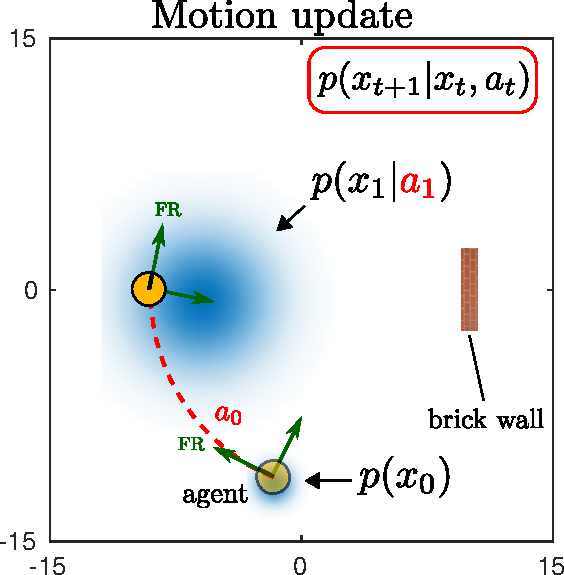
\includegraphics[width=0.45\textwidth]{/home/guillaume/Documents/Thesis/ch2-Background/Figures/motion_update.pdf}}
  \subfigure[]{\label{fig:measurement}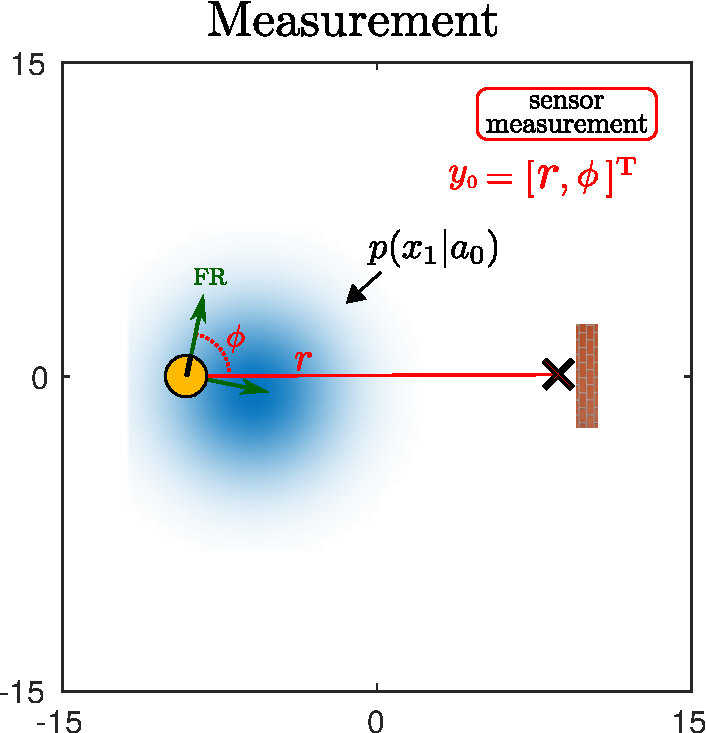
\includegraphics[width=0.45\textwidth]{/home/guillaume/Documents/Thesis/ch2-Background/Figures/measurement.pdf}} 
  \subfigure[]{\label{fig:likelihood}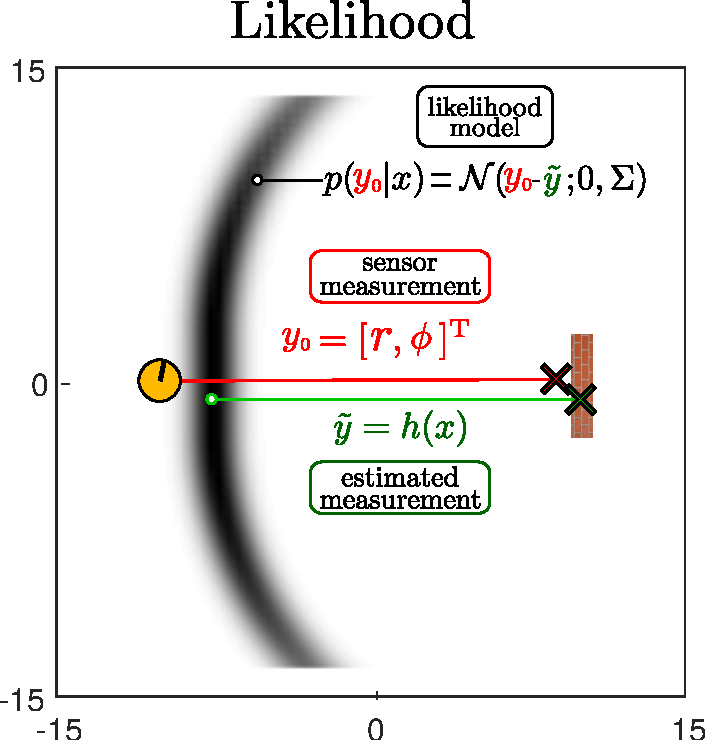
\includegraphics[width=0.45\textwidth]{/home/guillaume/Documents/Thesis/ch2-Background/Figures/likelihood.pdf}} 
  \subfigure[]{\label{fig:measurement_update}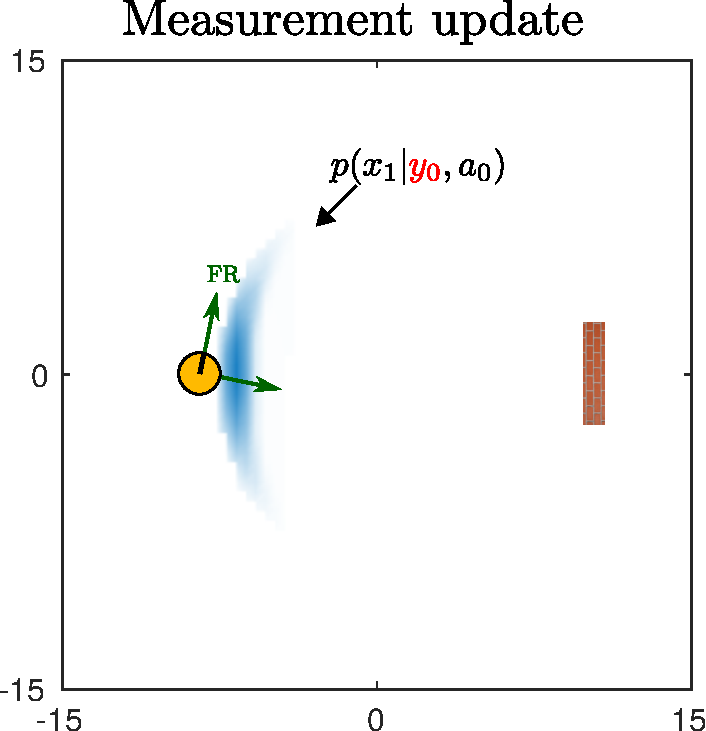
\includegraphics[width=0.45\textwidth]{/home/guillaume/Documents/Thesis/ch2-Background/Figures/measurement_update.pdf}} 
 \caption{\textbf{(a)} An agent is located to the south west of a brick wall, it is equipped with a 
  range sensor. The agent takes a forward action, but skids which results in a high increase of the uncertainty.\textbf{(b)} 
  The agent takes a measurement, $y_0$, of this distance to the wall; because his sensor is noisy his estimate is off. 
  \textbf{(c)} The agent uses with his measurement model to evaluate the plausibility of all locations in the world which would result in a similar
  measurement; illustrated by the likelihood function $p(y_0|x_0)$. \textbf{(d)} The likelihood is integrated into the probability 
  density function; $p(x_0|y_0) \propto p(y_0|x)p(x_0)$.}
  \label{fig:belief_update_example}
\end{figure}

In Figure \ref{fig:belief_update_example} \textbf{(c)} the likelihood is illustrated; the dark regions indicate areas of high 
likelihood, which are possible locations from which the sensor measurement could have originated from. The value of the measurement
likelihood function is then integrated into the state space probability density function.

These two steps: \textbf{motion}  and \textbf{measurement} updates are part of a state estimation process called a \textbf{Bayesian state space filter}, 
which we formalise below in Equation \ref{eq:motion_update}-\ref{eq:measurement_update}.
\begin{figure}
\centering
\begin{tikzpicture}
\node [white_box] (box){%
     \begin{minipage}{0.9\textwidth}
     The Bayesian filter turns a prior probability distribution over the state space, $p(x_t|y_{0:t-1},a_{0:t-1})$,
  to a posterior $p(x_t|y_{0:t},a_{0:t})$ by incorporating both motion and measurement. Applied recursively it 
  keep a probability distribution over the state space which considers all the past history of actions and observations.We define 
  the application of these two steps by the filter function $\tau$, which returns takes the current belief, applied action 
  and measurement to return the next belief, $b_{t+1}$.\\
  
  \textbf{Motion update}
	\begin{equation}\label{eq:motion_update}
	  p(x_t|y_{0:t-1},a_{0:t}) = \int p(x_t|x_{t-1},a_{t-1})\, p(x_t|y_{0:t-1},a_{0:t-1})\;da_{t-1}
	\end{equation}
      \textbf{Measurement update}
	\begin{align}\label{eq:measurement_update}
	  p(x_t|y_{0:t},a_{0:t})   &= \frac{1}{p(y_t|y_{0:t-1},a_{0:t})}p(y_t|x_t)\,p(x_t|y_{0:t-1},a_{0:t}) \\
	  p(y_t|y_{0:t-1},a_{0:t}) &= \int p(y_t|x_t)\,p(x_t|y_{0:t-1},a_{0:t}) dx_t
	\end{align}   
	\textbf{Filter function}\\
	\begin{equation}
	  b_{t+1} := \tau(b_t,a_t,y_t) 
	\end{equation}
    \end{minipage}
};
\node[fancytitle, right=10pt] at (box.north west) {Bayesian filter};
\end{tikzpicture}%
\caption{Bayesian state space filter.}
\end{figure}

The motion model, Equation \ref{eq:motion_update}, updates the position of the probability distribution according to 
the applied action, $a_t$, and adds uncertainty by increasing the spread of the distribution. The measurement information is 
the incorporated by Equation \ref{eq:measurement_update}. The measurement likelihood always decreases the uncertainty 
or leaves it constant. It never results in an increase of uncertainty. The Bayesian state space filter is such an important 
component to belief space decision making that we define it by the filter function, $\tau(b_t,a_t,y_t)$, which 
takes as input the current belief, applied action and sensed measurement and returns the resulting belief $b_{t+1}$.
The state space filter is an essential component to a POMDP as it will become apparent.

%Depending on the type of sensors: stereo cameras, infra red sensors, Kinect, 
%omnidirectional camera, etc.., there is uncertainty associated with it. It is thus important 
With the latent state and its relation to the observation variable and the Bayesian filter defined, we can introduce the POMDP model
in Figure \ref{fig:pomdp} (\textit{left}). It has the same markov chain structure 
present in MDP, introduced in the previous section, but the state space $X$ is latent and 
a new layer of observation variables $Y$ is present. 

\begin{figure}
 \centering
  \centering
  \subfigure[]{\label{fig:sub_pomdp}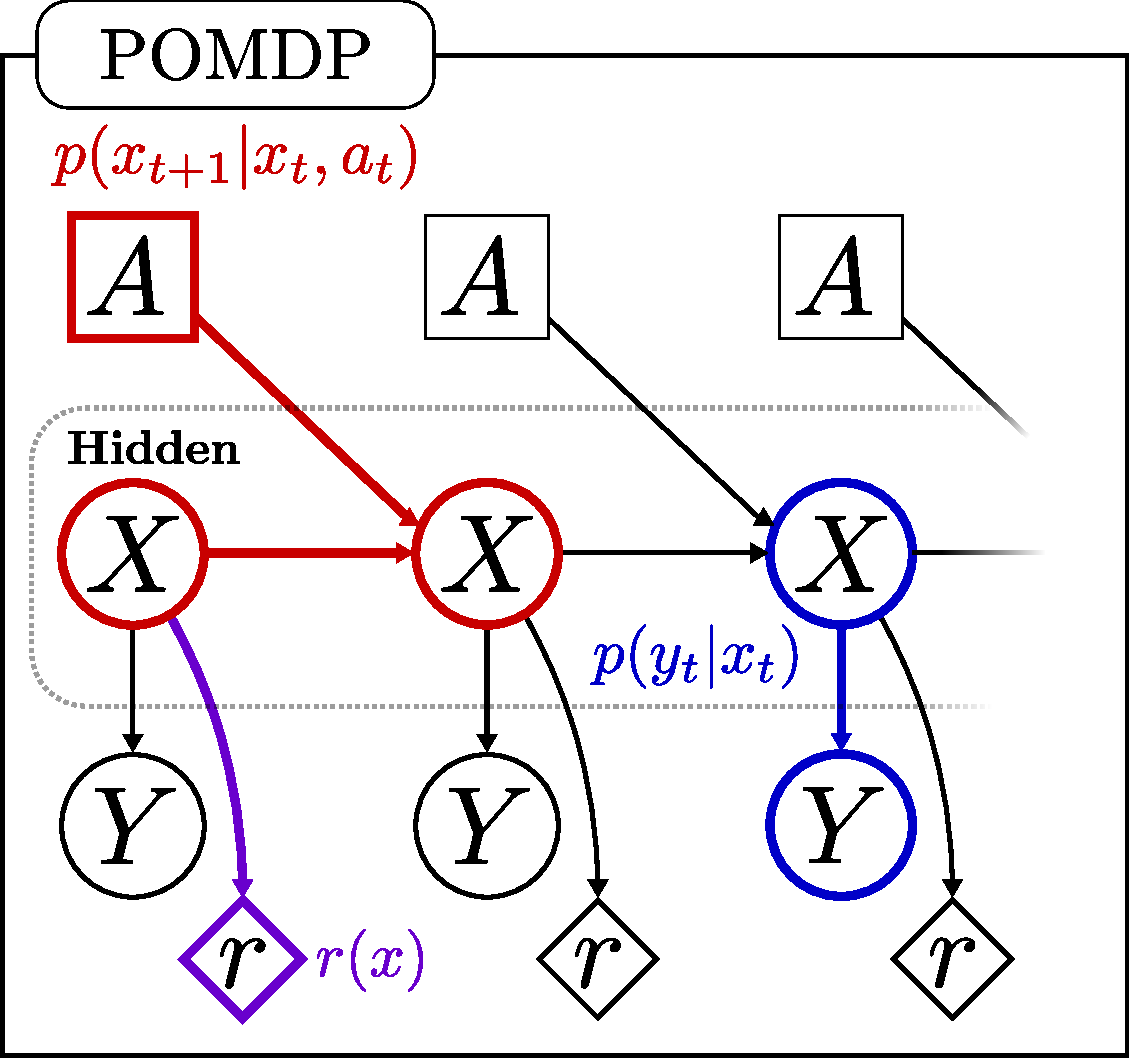
\includegraphics[width=0.45\textwidth]{/home/guillaume/Documents/Thesis/ch2-Background/Figures/pomdp2.pdf}}
  \subfigure[]{\label{fig:sub_bmdp}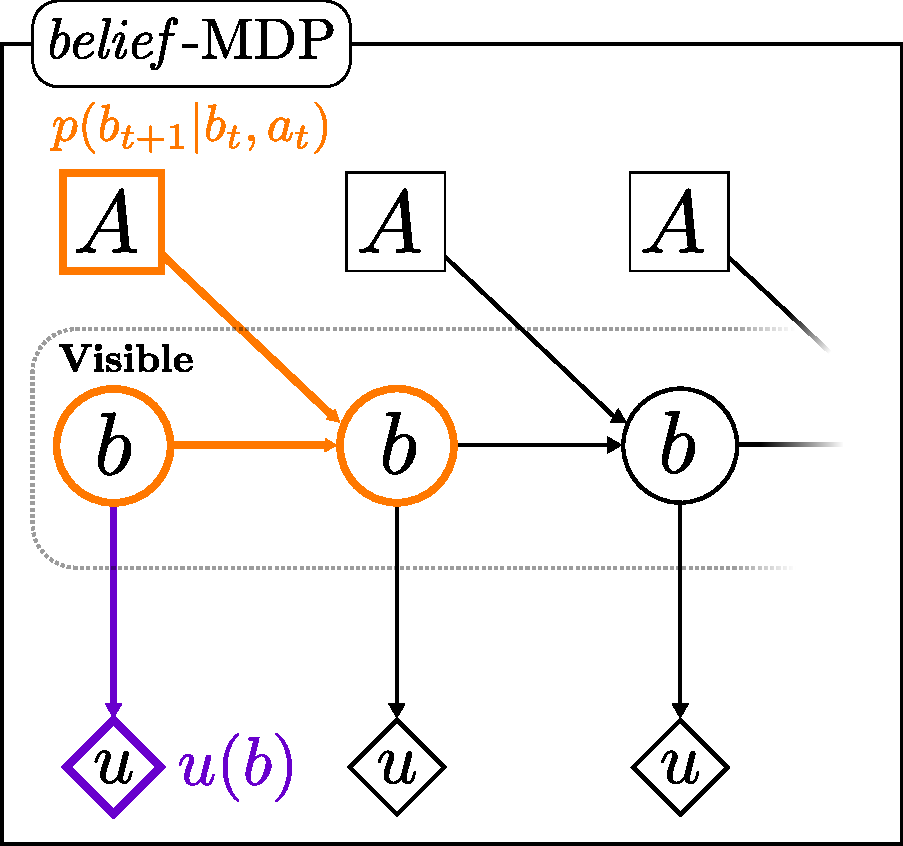
\includegraphics[width=0.45\textwidth]{/home/guillaume/Documents/Thesis/ch2-Background/Figures/pomdp3.pdf}} 
  \caption{\textbf{(a)} POMDP graphical model. The state space, $X$, is hidden, but is still partially observable through a 
  measurement, $Y$. \textbf{(b)} belief-MDP, the POMDP is cast into a belief Markov Decision Process. The state space is 
  a probability distribution, $b(x_t) = p(x_t)$, (known as a belief state) and is no longer considered a latent state. The original state 
  transition function $p(x_{t+1}|x_t,a_t)$ is replaced by a belief state transition, $p(b_{t+1}|b_t,a_t)$. The reward 
  is now a function of the belief.}
  \label{fig:pomdp}
\end{figure}

%We will see that because the state space is hidden it will cause complications to the maximisation of the expected utility.
%Since the states are not observable, the agent cannot choose its actions based on the state. The explicit 
%representation of the past events is typically memory expensive. Instead it is possible to summarize all relevant %
%information from previous actions and observations in a probability distribution over the state space, known as the
%belief state. 

Because the state space is partially observable the expected reward has to be computed for each possible history of states, actions and observations.
All approaches in the literature instead encapsulate all these possible histories into a belief state $b(x_t)$ (for short notation $b_t$)
which is a probability distribution (also referred to as an information state, \textit{I}-state) over the state 
space $x_t$ and use this new state description to cast the POMDP into a \textbf{belief-MDP} (states are probability distributions, 
beliefs). By casting the POMDP to a \textit{belief}-MDP the state space is considered observable and we recover the same structure 
as in the standard MDP problem.

Because we are working with in a belief-space the reward function has to be adapted to:
\begin{equation}
  r(b_t) = \int_{x_t} r(x_t)\, b(x_t)\;dx_t
\end{equation}
which is the expected reward $r(b_t) = \mathbb{E}_{b_t}\{r(x_t)\}$. The goal as before is to find a sequence of actions 
which will maximise the expected utility. Since our \textit{belief}-MDP has the same structural form as the MDP the solution 
to the problem is the same bellman equation equation derived previously. We just substitute the new belief transition function 
and we get the corresponding belief bellman Equation, \ref{eq:belief_bellman}.
\begin{equation}\label{eq:belief_bellman}
 V^*(b_t) = r(b_t) + \gamma \max_{a_t} \int_{b_{t+1}} p(b_{t+1}|b_t,a_t)\,V^*(b_{t+1})\;db_{t+1}
\end{equation}
Using this equation in this form is problematic, we are integrating over the space of beliefs and the 
transition function is a probability distribution over beliefs. The key to overcome this problem is to 
realise that if we know what the current measurement and applied action are there is only one valid possible belief.
Thus the integration over beliefs vanishes. This can be seen by substituting the belief transition function,
Equation \ref{eq:belief_state_transformation}, into the bellman equation Equation \ref{eq:belief_bellman}.
\begin{equation}\label{eq:belief_state_transformation}
 p(b_{t+1}|b_t,a_t) = \int_{y_t} p(b_{t+1}|b_t,a_t,y_t)\,p(y_t|y_{0:t-1},a_{0:t})\; dy_t
\end{equation}
After the substitution and re-arrangement of the sums we get an integral over all future value 
functions weighted by there probability, see Equation \ref{eq:max_component} which is the section of the bellman equation 
after the max. Since the observation is known (because the outer integral is over $y_t$),
the integral over the beliefs vanishes since there is only one possible future belief which is given by the 
Bayesian filter function $\tau(b_t,a_t,y_t)$.
\begin{equation}\label{eq:max_component}
 \gamma \max_{a_t} \int_{y_t} \underbrace{\left( \int_{b_{t+1}} p(b_{t+1}|b_t,a_t,y_t)\,V^*(b_{t+1})\; db_{t+1}\right)}_{1 \cdot V^*(\tau(b_t,a_t,y_t))}\, p(y_t|y_{0:t-1},a_{0:t}) \; dy_t
\end{equation}
In the final belief state bellman equation, the integral of the belief state is replaced by an integration over observations,
Equation \ref{eq:final_belief_bellman}.
\begin{align}\label{eq:final_belief_bellman}
  V^*(b_t) &= r(b_t) + \gamma \max_{a_t} \int_{y_t}  p(y_t|y_{0:t-1},a_{0:t}) \,V^*(f(b_t,a_t,y_t))\; dy_t \nonumber  \\ 
	   &= r(b_t) + \gamma \max_{a_t} \E_{y_t}\{V^*(f(b_t,a_t,y_t))\}
\end{align}
The belief bellman equation is intuitive, the value of the current belief is the immediate reward plus the value of the 
future belief states weighted by the probability of a measurement which would result in these future belief states. 
It turns out that computing a value function using the above bellman function is not computationally tractable. Solving 
a POMDP problem as for the MDP case consists of finding the optimal value function from which the optimal policy can 
be derived. Essentially the same dynamic programming and reinforcement learning techniques can be applied to solve 
this problem. An exact solution is however only  feasible when considering a finite state, action and observation space and
a finite planning horizon $T$. Most early techniques for solving POMDPs used value iteration. It has been shown (\cite{Sondik_1973}) 
that because the reward function uses a linear operator (the expectation) and that the bellman backup operation 
(applying the bellman equation to the current value function) preservers the linearity, the value function after each 
updates is piece wise linear and continuous (PWLC). The intractability comes from the successive applications 
of the bellman backup operation which result in an exponential time and space complexity with respect to the planning horizon.
A good text on the implementation of exact value iteration for POMDPs can be found \cite[Chap. 15]{Thrun_2005}
and here \cite{Kaelbling_1998}.

%From considering the decision belief tree of the POMDP, Figure \ref{fig:pomdp_bel_tree}, we can appreciate the complexity of the problem
%of finding an optimal policy. Given a discrete set of actions and observations to update the belief $b_1$ we have to consider a time 
%complexity of $\mathcal{O}(|U||Y|^T)$ where $T$ is the depth of the tree (the planning horizon). Given that we have a finite set of 
%belief the complexity solving the POMDP is $\mathcal{O}(|\mathcal{B}||U||Y|^T)$. 


%\begin{figure}[h]
% \centering
% 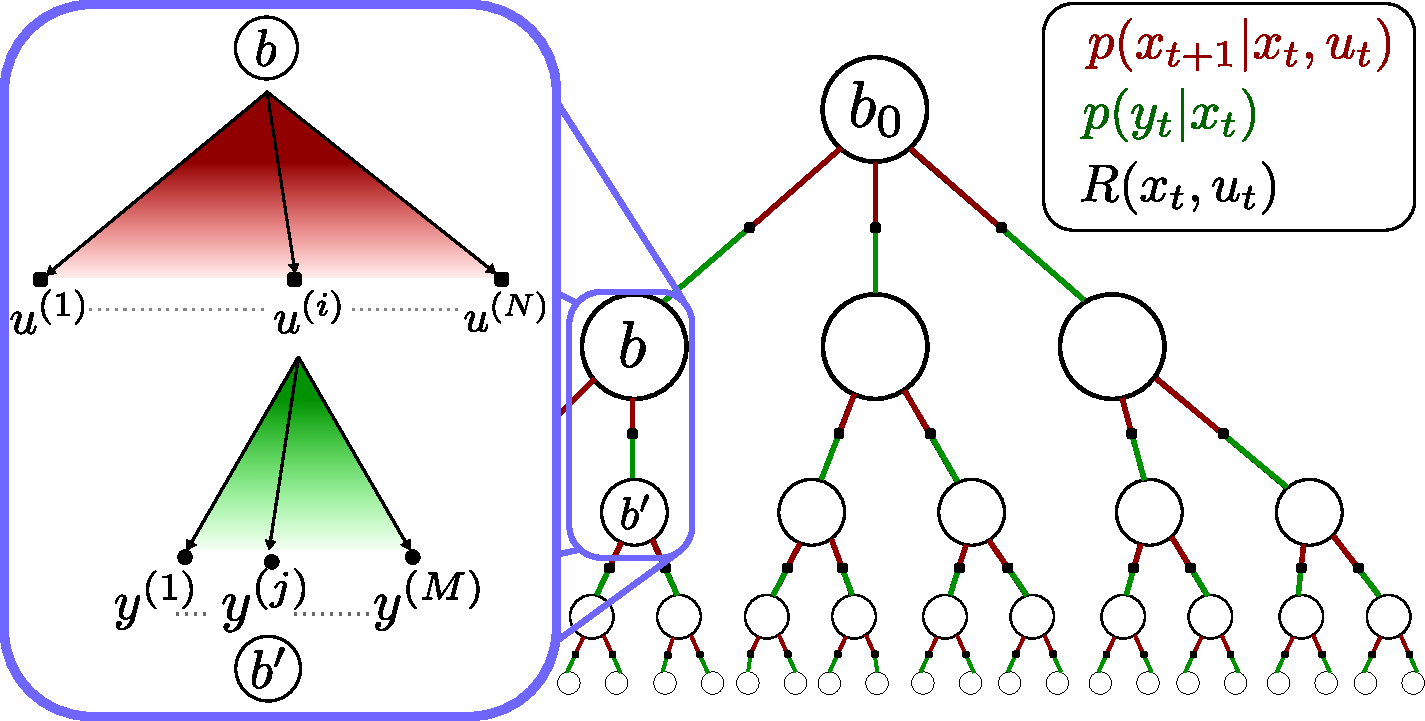
\includegraphics[width=\textwidth]{/home/guillaume/Documents/Thesis/ch2-Background/Figures/belief_tree.pdf}
%  \caption{ad}
%\end{figure}

Why is POMDP so good: combine information gathering and goal directed actions in one. Give taxonomy of planning under uncertainty here.
Finding a a solution to a POMDP is PSACE-complete (Papadimitriou & Tsitsikis, 1987), even when 
the dynamics are known. Thus approximate methods are needed for even the simplest problems.

\section{State of the art}

We review the latest methods of solving sequential decision problems under uncertainty. This is an extremely dense and spread out 
area of research, no doubt because of its importance and the fact that it cannot be ignored. If uncertainty is not considered 
adequately, the control policy risks being suboptimal or lead to drastic failure. 




\subsection{Point-based Value Iteration}

The POMDP formulation introduced previously is the main theoretical starting point of policies which
consider uncertainty. However solving an exact POMDP, problem through dynamic programming (value iteration) is 
computationally intractable and an exact solution only exists for discrete state, action and observation space \cite[Chap. 15]{Thrun_2005}.
This intractability, in which only problems with a few states could be solved, inhibited the application of the POMDP framework to robotics. 
The first breakthrough, Point-Base Value Iteration (PBVI) \cite{PBVI}, allowed to apply VI to a robotic navigation problems (626 states). The key insight 
which allowed VI to scale was to only consider a subset of the belief states which were reachable and relevant to the problem. This is achieved by smart sampling techniques
and only perform VI backups on beliefs states which are relevant. Before this point and before only value iteration on this subset instead of considering all beliefs.  If you 
have a $10 \times 10$ gird, this results in a total of a $100$ states and a belief state of a $100$ dimensions! The PBVI approach initiated a renewed effort in 
porting VI to POMDPs with larger and larger state spaces. From this point most research as focused on determining efficient strategies to sample belief points and
which to backup via VI. Heuristic Search Value Iteration (HSVI1) (\cite{HSV}) and HSVI2 (\cite{HSVI2}) uses forward search heuristic to find relevant beliefs by keeping a lower and upper 
bound on the current estimated value function. The belief tree gets expanded by choosing the action and observation whilst considering there potential future effect
on the value of the bounds, which thy try to minimise. It has equivalent results than classical PBVI with an exception to game of tag problem in which it fairs 
significantly better.  Later, Forward Search Value Iteration (FSVI) (\cite{FSVI}) takes an alternative approach than keepings an upper and lower bound on 
the value function, because doing so results in a drastically increases in the computation time necessary to find a solution. Instead they assume that the 
state space is fully observable, solve the the MDP problem and use this policy in the POMDP setting to generate a set of beliefs. It is orders of 
magnitude faster than HSVI and results in comparable polices. FSVI fairs badly however when information gathering actions are necessary. Since it is 
essentially using a myopic policy to generate it samples, these will be insufficient to find the global optimal policy when the solution requires 
information gathering actions. One of the very last sampling generation techniques which is considered to be the most efficient is SARSOP (\cite{SARSOP}),
it uses aspects present in both upper and lower bounds on the value function and the equivalent uncertainty free MDP solution to the problem. It tries
to sample belief points which will contain the optimal set of samples necessary to achieve an optimal policy.  Both SARSOP and HSVI2 are considered 
state of the art in PBVI value approximation techniques. (See \cite{POMDP_approach_2010}) for a review and comparison of both techniques on problems 
with thousands of states including simulation examples in grasping, tracking and UAV navigation. 

These methods are well suited to address problems which are easily expressed in a discrete state space. All considered problems are simulation based and 
no physical interaction problems are considers. Besides the belief set generation problem, interest has also been poised on porting the PBVI to a continuous state space.
A example of a continuous action space PBVI method is Perseus \cite{Spaan05icra}, in which the authors replace the maximisation over the action by instead sampling them from a 
parametric continuous representation. In \cite{PBVI_C_2006} the state space, transition and observation model are represented by Gaussian Mixtures and the authors consider a particle 
set or Gaussian mixture representation of the belief. The authors show that a continuous representation of the state space preserves the PWLC property of the value function. They extend 
there method to continuous action and observations through a sampling instead of discretising. Results are shown in 1D continuous corridor setting. In a 
more recent approach \cite{solving_continous_pomdps_2013} a discrete state presentation of a continuous state space is learned and is combined with sampling
techniques to solve the continuous integrals present in the bellman equation. The explicit learning of the state representation lead to an increased performance
when compared to the other continuous state PBVI methods and the others considered both continuous state and observation space. 

PBVI techniques have come fare since their first application to robotics navigation back in 2003 and have lead to a rapid increase of interest. 
Initially only a few hundred states could be considered and now problems with over ten thousand states are being solved in seconds. 
Most of the research has focused on how to gather efficiently a good set of sample beliefs. Later there have been efforts to expand PBVI 
to continuous state spaces such to be more suited to robotic applications. The main approach consists of using sampling techniques to overcome 
the maximisation over the actions (when considering continuous actions) or to choose a suitable parametric representation of the transition, observation 
and reward model such that the bellman equation can be solved in closed form. Most evaluation of have focused on simulated and simplified robotic 
navigation problems in 1D and 2D. We have not discussed online POMDP-solvers since there also based on VI and sampling techniques and thus share 
a lot of similarities with PBVI, we refer the reader to \cite{Ross08onlineplanning} for a detailed review.

%\cite{MCVI_CS_POMDPs}	% sampling techniques 

%Resent advances in PBVI methods: \cite{Veiga14aaai} 	   % Pedro Lima Point-Based method for Factor value 

% Point-based Value Iteration for Continuous POMDPs

\subsection{Parametric Value Iteration}

Point-based Value Iteration techniques tried to preserve the PWLC property of the value function. This directly 
leads to a discretization of the state space which if continuous by nature leads use prone to the curse of dimensionality.
An alternative approach is to represent the belief space by a parametric representation, for instance as a Gaussian function. 
The value function is then defined as a function of the parameters of the Gaussian. This approach in effect greatly 
diminishes the dimensionality problem but does away with the PWLC property of the value function. Instead to generalise 
the value of particular parameter a regressor function is needed and to learn it approximate dynamic programming techniques 
are used.

A very first successful example of this approach is \cite{MC-POMDP} were a POMDP problem in a continuous 
state, action and observation space was solved; with a working implementation on a physical mobile base.  
The belief was represented by a particle filter and the policy by a Q-value function, whose functional form was 
a non-parametric regressor (k-nearest neighbour) of the particle filter. The distance metric was the sample KL divergence
between two particle sets. The POMDP was solved through Reinforcement Learning (interaction with the environment) and 
approximated dynamic programming also known as experience replay, batch RL or Fitted Q-Iteration (FQI) \cite{Tree_batch_2005}. 
Although highly computationally demanding the method was successful. 

This lead to many similar approaches such as \cite{mc_update_ppomdps} where the belief state filter was an 
Extended Kalman Filter (EKF), the value function was also non-parametric and the POMDP was solved via FQI. 
When compared with Perseus in a discretized 2D localisation task both approaches reached equivalent 
policies but the authors method achieved it much faster than Perseus, a PBVI method. 

% 1) Belief space compression and value iteratrion
Another similar approach to parametrising the belief is to compress it to sufficient statistics and treat 
the decision problem as a fully observable augmented MDP (AMDP) in this new state representation. In \cite{Roy99coastalnavigation}
the authors compress the filtered belief to its mean and entropy and performed VI on this augmented state space
in a navigation task in which the goal was to reach a location with a minimum amount of uncertainty. This approach
brings a great simplification to solving the POMDP by at the cost of a lossy belief compression. In further developments
\cite{belief_compression_2005} compared both PCA and exponential-PCA (E-PCA, \cite{EPCA_2003}) as a means of belief compression techniques to find a low
dimensional belief space. This approach showed to be superior than the AMDP, it however requires transitioning back and forth 
between the low and high dimensional belief states. A step necessary for the the application of VI. The latest work in this 
area is \cite{bs_compression_2010} which investigates the use of nonnegative matrix factorisation in combination of k-means 
clustering as a means of compressing the belief which showed some improvement over the E-PCA approach but was only evaluated 
on discrete benchmark problems. Belief compression as mean of reducing the complexity of the belief state is interesting. The 
down side is that it requires discretising the belief to a fixed non-dynamic grid, collected many samples and learn an 
appropriate set of belief-basis eigenvectors. As such the larger the state space, the larger the dimensionality and thus more
samples are required to find a suitable set of basis.

% 2) A very large state space and do away with 
Recent developments lean more to the idea of very large state space representation and treat the problem as a MDP. In contrast to 
POMDPs there has been fare more research focused on MDPs and a lot of work has been done on the application of non-linear function 
approximators for representing the value function in combination with reinforcement learning optimisation techniques to solving them.
A successful example was the the usage of a multi-layer perceptron as a Q-value function approximator, Neural Fitted Q-Iteration (NFQ) \cite{neura_fqi_2005}.
This approach was successfully applied to the standard RL benchmarking problems (carte pole, acrobat, mountain care), but no partially observable
setting was considered. It is later in \cite{DRQ_AAAI_2015} that authors applied a Deep Recurrent Q-Network (DRQN) (extension to the work in \cite{mnih-dqn-2015})
to capture the history of states in a game of Pong where the state space was occluded half the time. By introducing a long term memory component 
the POMDP in effect is turned into a MDP and the authors apply an optimisation approach similar to FQI. 

Parameterization of the belief is a way of reducing the curse of dimensionality. By doing so the VI solution is no longer closed form and
function approximators are need to represent the value function. The value function is then optimised via approximate dynamic programming 
or reinforcement learning. These approaches are considerably more simple to implement than PBVI solvers which require heuristic pruning 
techniques and are difficult to port to continuous state spaces in general. There is a tendency to represent the POMDP has an augmented state MDP 
which then allows to apply well developed RL techniques. By using advanced non-linear function approximators the large state spaces can be 
handled in an efficient way and optimal policies can be found. However most of the applications seen so fare do no consider continuous actions
at all. Even for standard MDP the application of continuous action is problematic, which is due to need to maximise over the actions. We next
review a third approach of dealing with POMDPs which is more adapted to continuous actions. 

\subsection{Policy search}

The approaches seen so fare use a vale function to encode the problem which when solved a policy can be derived from it.
This requires learning a high dimensional value function over the belief space and the resulting policies are not necessarily 
smooth. This is because small changes in the value function can lead to drastic changes in the policy [cite]. There is no 
doubt that deriving a policy from a generic value function for highly continuous policy such in the case of controlling an
articulated robotic arm is no easy task. 
This has lead to development of an alternate approach in which a policy is learned directly without a value function. Instead
an initial policy is defined in terms of a parametrised function, $\policy$, and the utility is a function of the parameters, 
$u(\boldsymbol{\theta})$. The optimal policy is found by searching for the parameters $\boldsymbol{\theta}$ which will maximise 
the utility function. This is can be accomplished through various optimisation methods: gradient descent, expectation-maximisation, etc...

% Policy Iteration
%Early work include the application of policy iteration to a finite state controller \cite{p_search_pomdp_1998}. A finite state controller
%is iteratively evaluated (VI) and then subsequently improved until an optimal policy is found. Evaluation of the policy is much faster 
%than solving the optimal bellman equation, since the maximisation over the actions is absent. 

% Reinforce (gradient based methods)

% Actor-critic methods (combine both value function and policy)

% REINFORCE - PoWER - PI2 - 
One of the very first applied class of policy search algorithms were the REINFORCE (likelihood ratio) algorithms
first introduced by Williams \cite{reinforce_1992}. From a set of example episodes, also called roll-outs, the gradient
is estimated. The key aspect to this approach is that the derivative of the cost function is independent of the state
transition model and as a result the gradient is easier to estimate from samples. Application of this methodology 
to a partially observable setting lead to Gradient POMDP, GPOMDP \cite{gpomdp_2000} in which the authors developed 
a conjugate stochastic gradient ascent algorithm to optimise a policy with respect to the average reward. 

\cite{sis_pomdp_2002}


\cite{PoWER_2009}
\cite{NAC_2008}

%  Basically do gradient descent on parameters
\cite{Pegasus_2000}
\cite{heli_2004}

\cite{RL_robots_surv_2013}
\cite{p_search_surv_2011}

\cite{dmp_seq_2012} % PI2
\cite{dmp_iros_2011}


% Non pomdp method %Heurisitc: Information Gain
\cite{dense_entropy_icra_2014}
% Policy search
\cite{Uncer_reduction_heuristic_2015}
\cite{Sol_POMDP_Policy_space_1998}

\cite{sigma_hull_iros_2013}
\cite{int_motion_planning_2013}  % belief space planning


\subsection{Heuristics}

% Generic planning under uncertainty (not directly using a policy representation)
\cite{next_best_touch}
\cite{CostalNavigation1999}

\subsection{Planning}
$b = (\mu,\Sigma)$
\cite{Quadrator_2008},
\cite{BelRoadMap_2009}

\cite{non_gauss_bel_plan_2012}	% Non-Gaussian belief space planning
\cite{active_RSS_07} 	% Active Policy Learning for robot planning and exploration under uncertainty
\cite{plan_cont_bel_space_2015}
\cite{rob_online_bs_icra_2014}
\cite{bel_roadmap_2009}


\subsection{Optimal control}
$b = (\mu,\Sigma)$
 
\cite{plattRSS10} 	% Belief space planning
\cite{Erez10ascalable},
\cite{van_den_Berg_2012}, 
\cite{Platt-RSS-10}

 
% Grasping examples 
Grasping
\cite{u_aware_grasp_ICRA_2015}
\cite{learn_grasp_un_icra_2011}
\cite{seq_traj_replan_iros_2013}
\cite{Li_2015}

% Under water navigation examples

\cite{un_water_inspection_icra_2012}

% Continous

Optimal control methods represent the belief by a Gaussian function 

\cite{Bayesian_explor_exploit_2009}
% Sample based replanning
%\cite{Rand_belief_space_replanning} reference does not seem to exist
\cite{Macro_uncertainty_2011}

\section{Summary}




